\section{Content}

Let's now move to the analysis of the content.
The page that we analyze is \url{https://siciliangoodness.shop/padovaviaroma/}. 
In general we can see that the back button works very well. From each page where we are we can go back to the previous one.
An other important aspect is that we avoid the phenomenon of 'The lost in the navigation'. In fact, in the homepage, with the breadcrumbs, we always know where we are and the path that we follow. 

\begin{figure}[H]
	\centering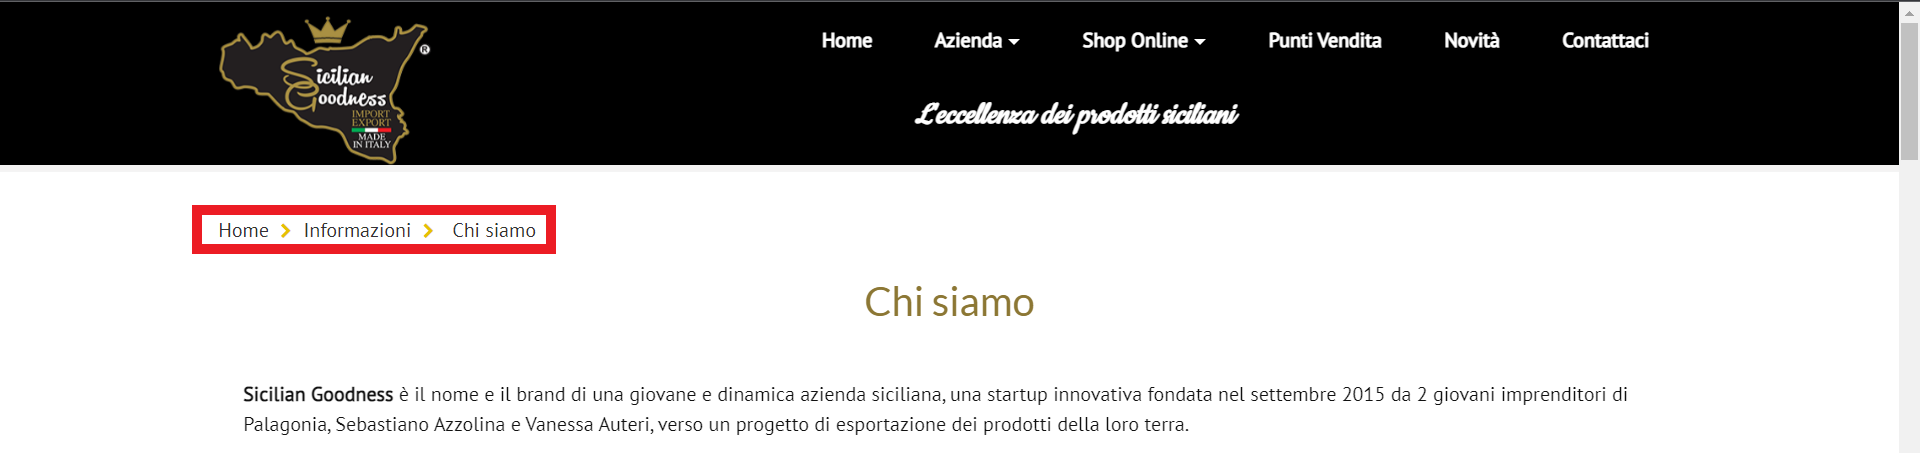
\includegraphics[width=12cm]{Img/bred2.png}
	\caption{Homepage Breadcrumb}
\end{figure}

The only pages that have some problems are 'SHOP VIGONZA' and SHOP PADOVA VIA ROMA'. Indeed, in these pages it is difficult to come back to the homepage, because it seems to be a new page where you start your research. We can see that no breadcrumbs are present and if we click on the logo we reload the same page. This is confirmed by the fact that if we click on a link (for example: 'VINI \& LIQUORI) we start the navigation from this page.

\begin{figure}[H]
	\centering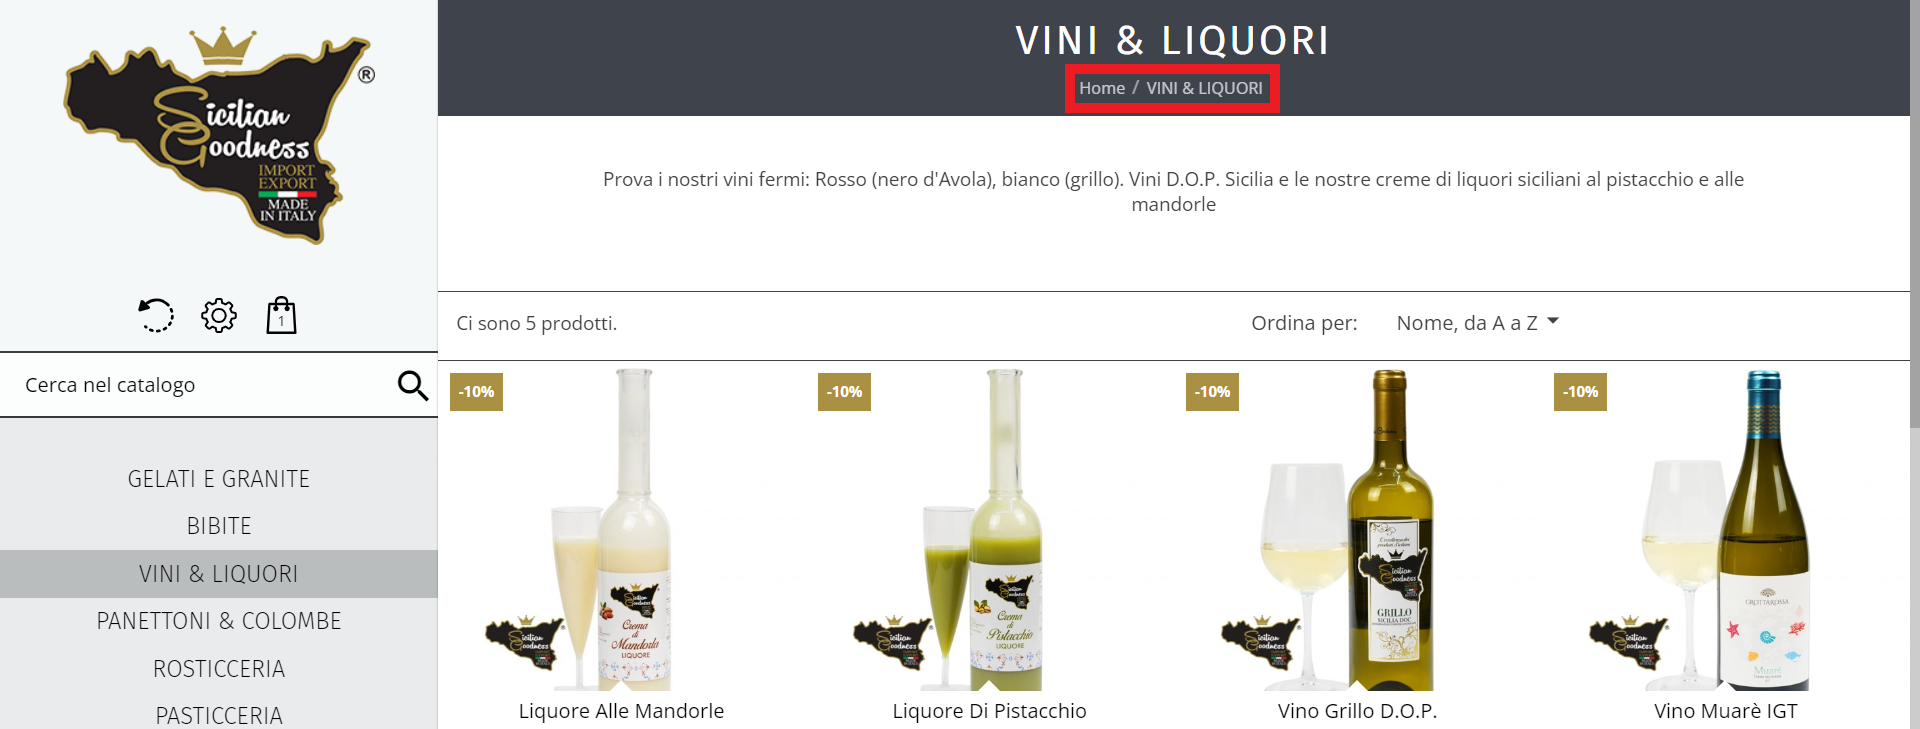
\includegraphics[width=12cm]{Img/bred1.png}
	\caption{Shop Breadcrumb}
\end{figure} 

In particular in this section we'll analyze the page to search the products and the 404 page will be briefly analyzed too. In conclusion we'll analyze the page of a single product (with the analysis of the Ws), as it is the most significant and most visited type of page.

\pagebreak

\subsection{Rest of the pages}
There is a lot of content in this page. In fact, for seeing all the information of the webpage we have to scroll more or less six times.
In the section \textbf{\hyperlink{sho}{First Page}} we analyze better some of the first elements. Now, we brefly see the content.

Immediately, we see that in the center there are all the information about the company(Who axis).

\begin{figure}[H]
	\centering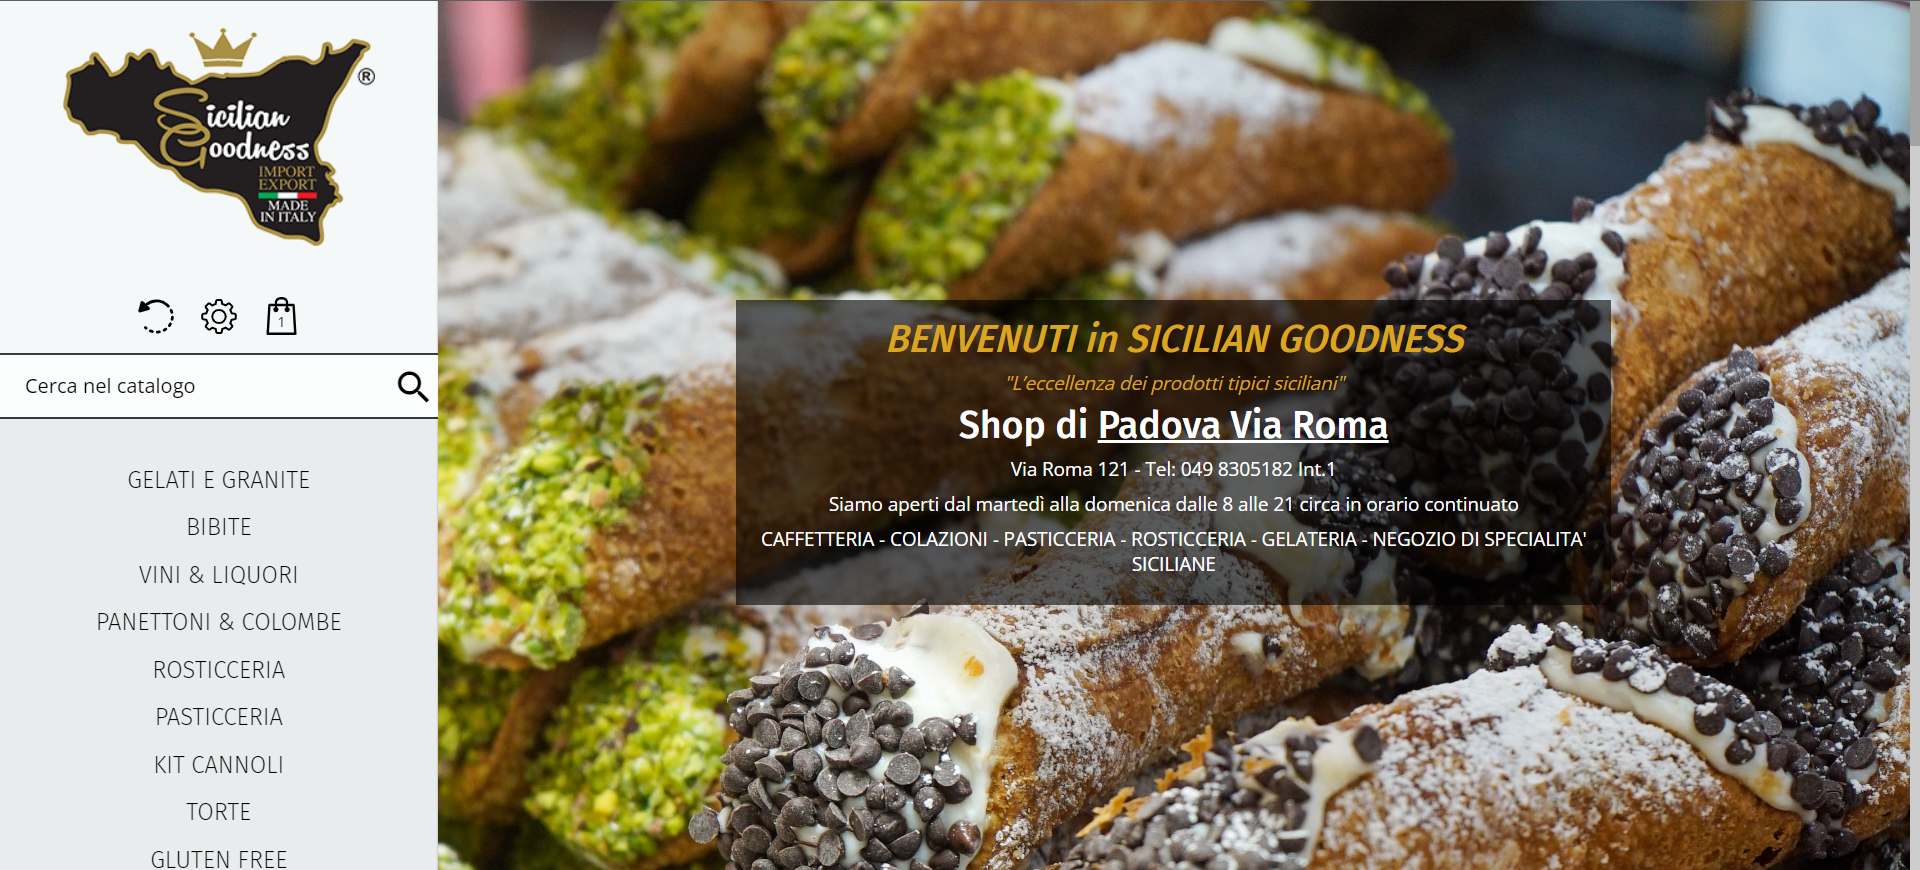
\includegraphics[width=12cm]{Img/con1.png}
	\caption{Content 1}
\end{figure}

In the second scroll we have a video to promote the shop. This can be a good method becuase videos require a low computational effort.

\begin{figure}[H]
	\centering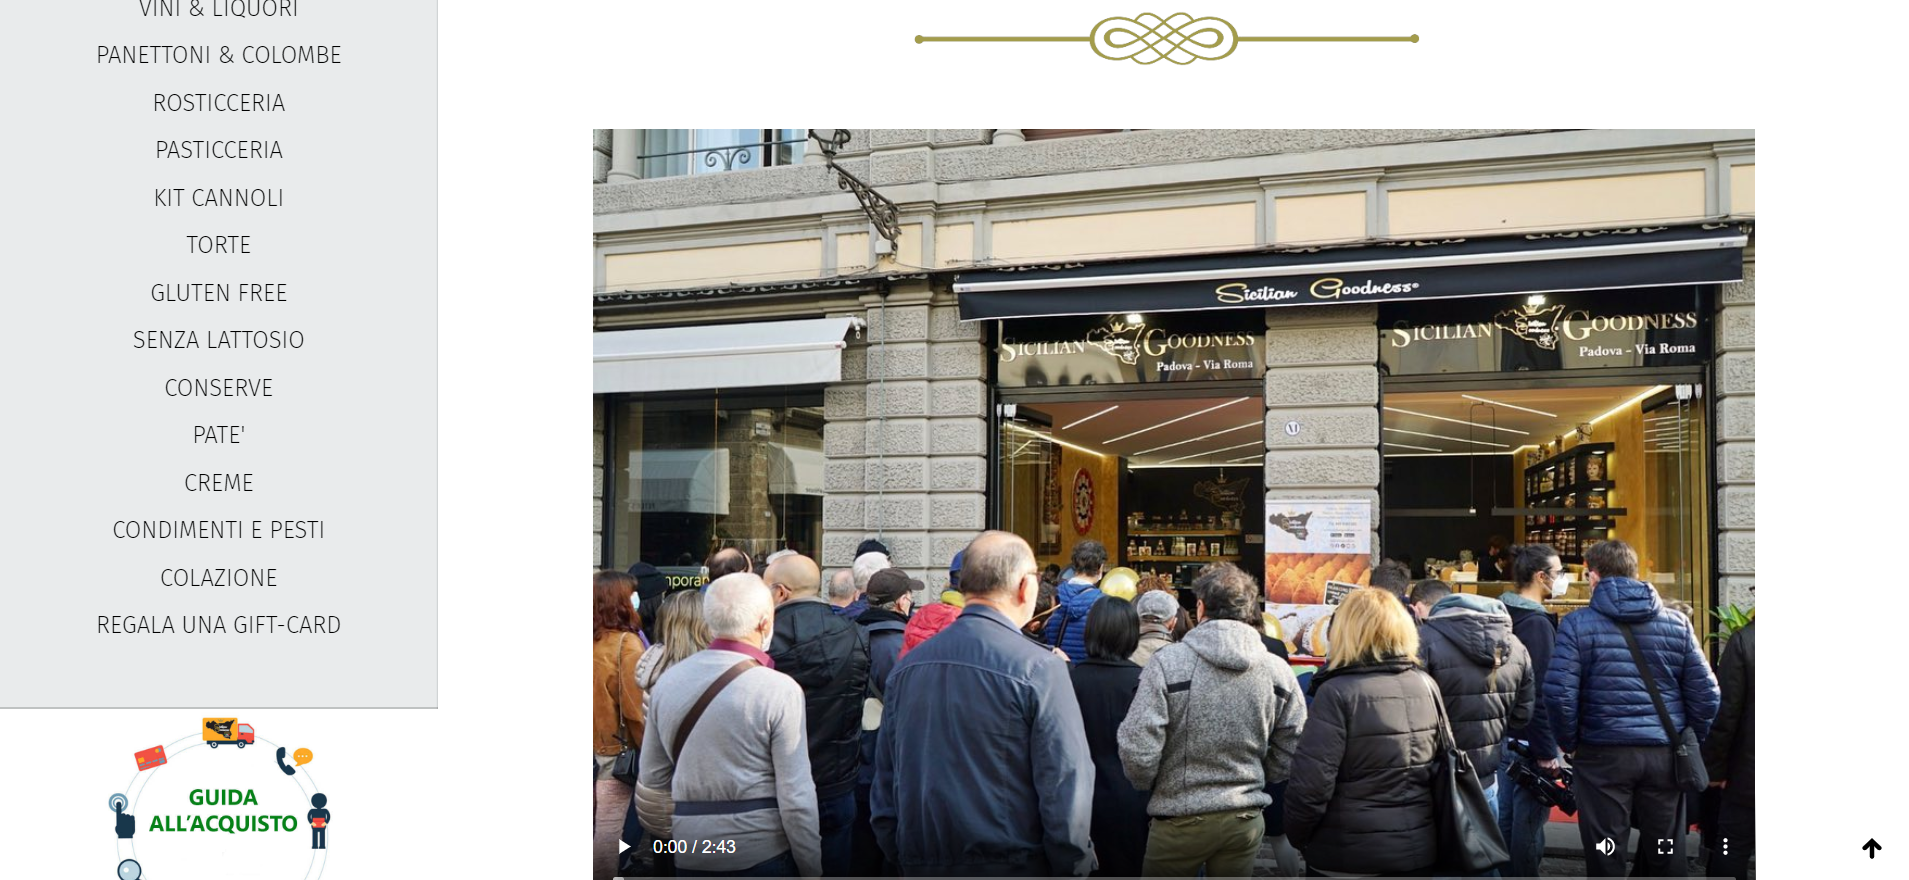
\includegraphics[width=12cm]{Img/con2.png}
	\caption{Content 2}
\end{figure}

\pagebreak

In the third scroll we have some advertisement.

\begin{figure}[H]
	\centering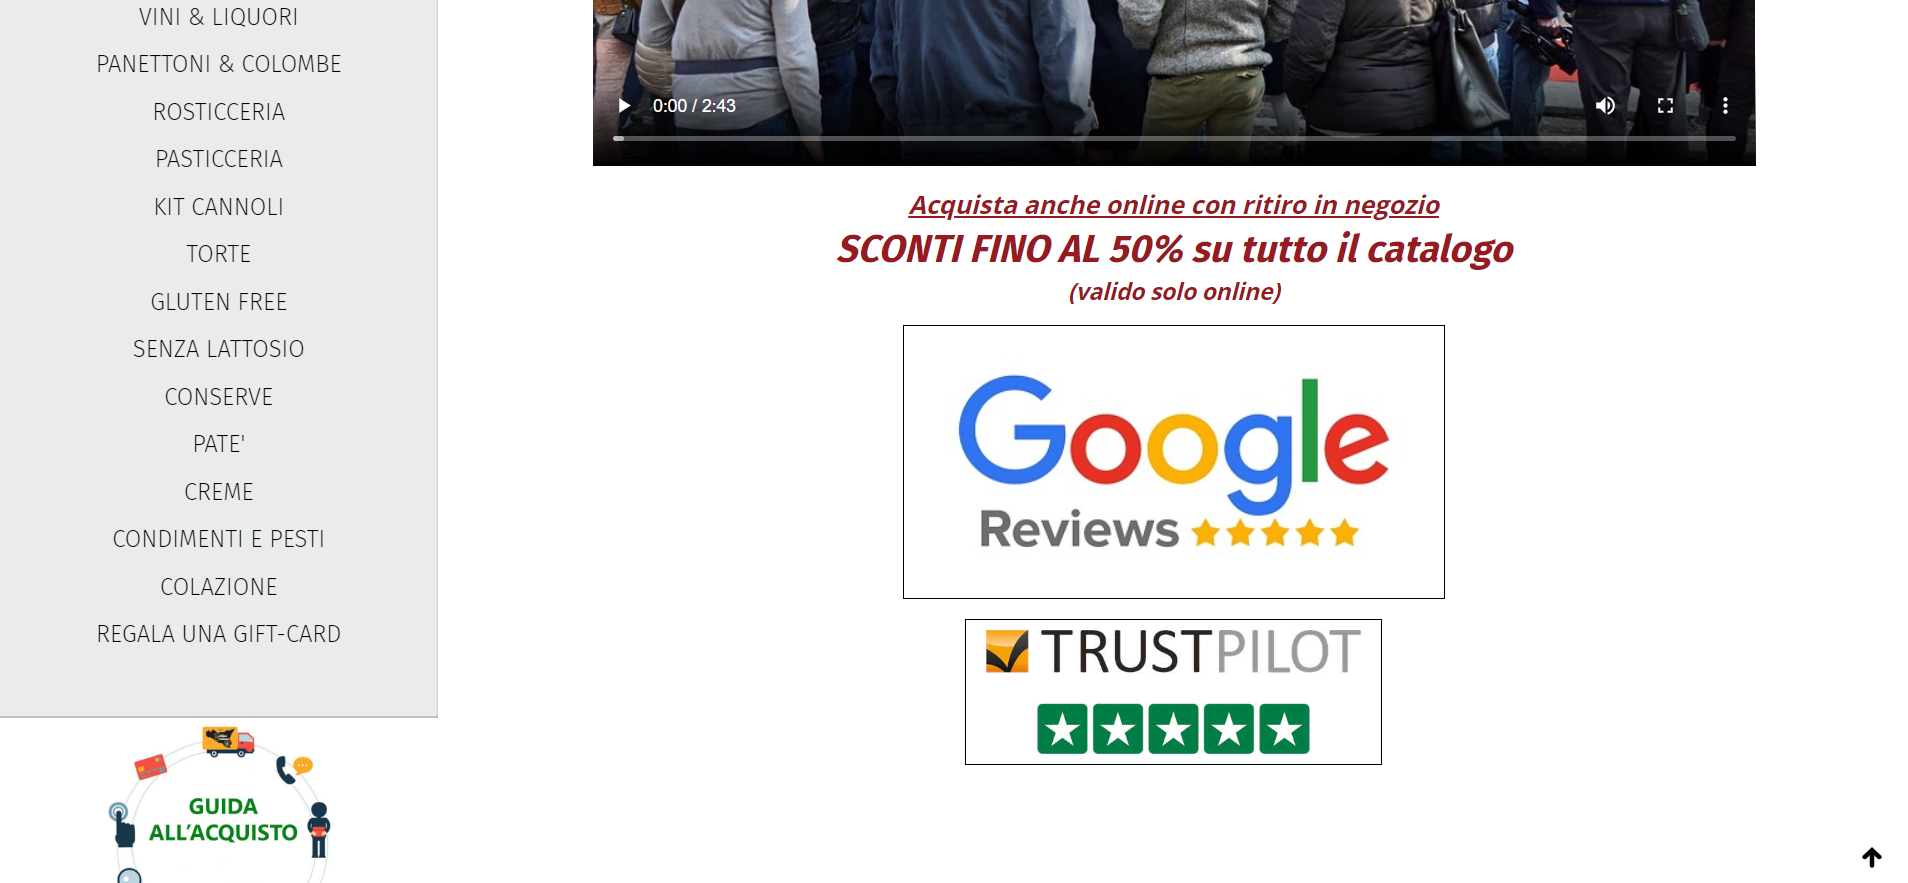
\includegraphics[width=12cm]{Img/con3.png}
	\caption{Content 3}
\end{figure}

In the fourth scroll we have some popular products in order to help users in the choice.

\begin{figure}[H]
	\centering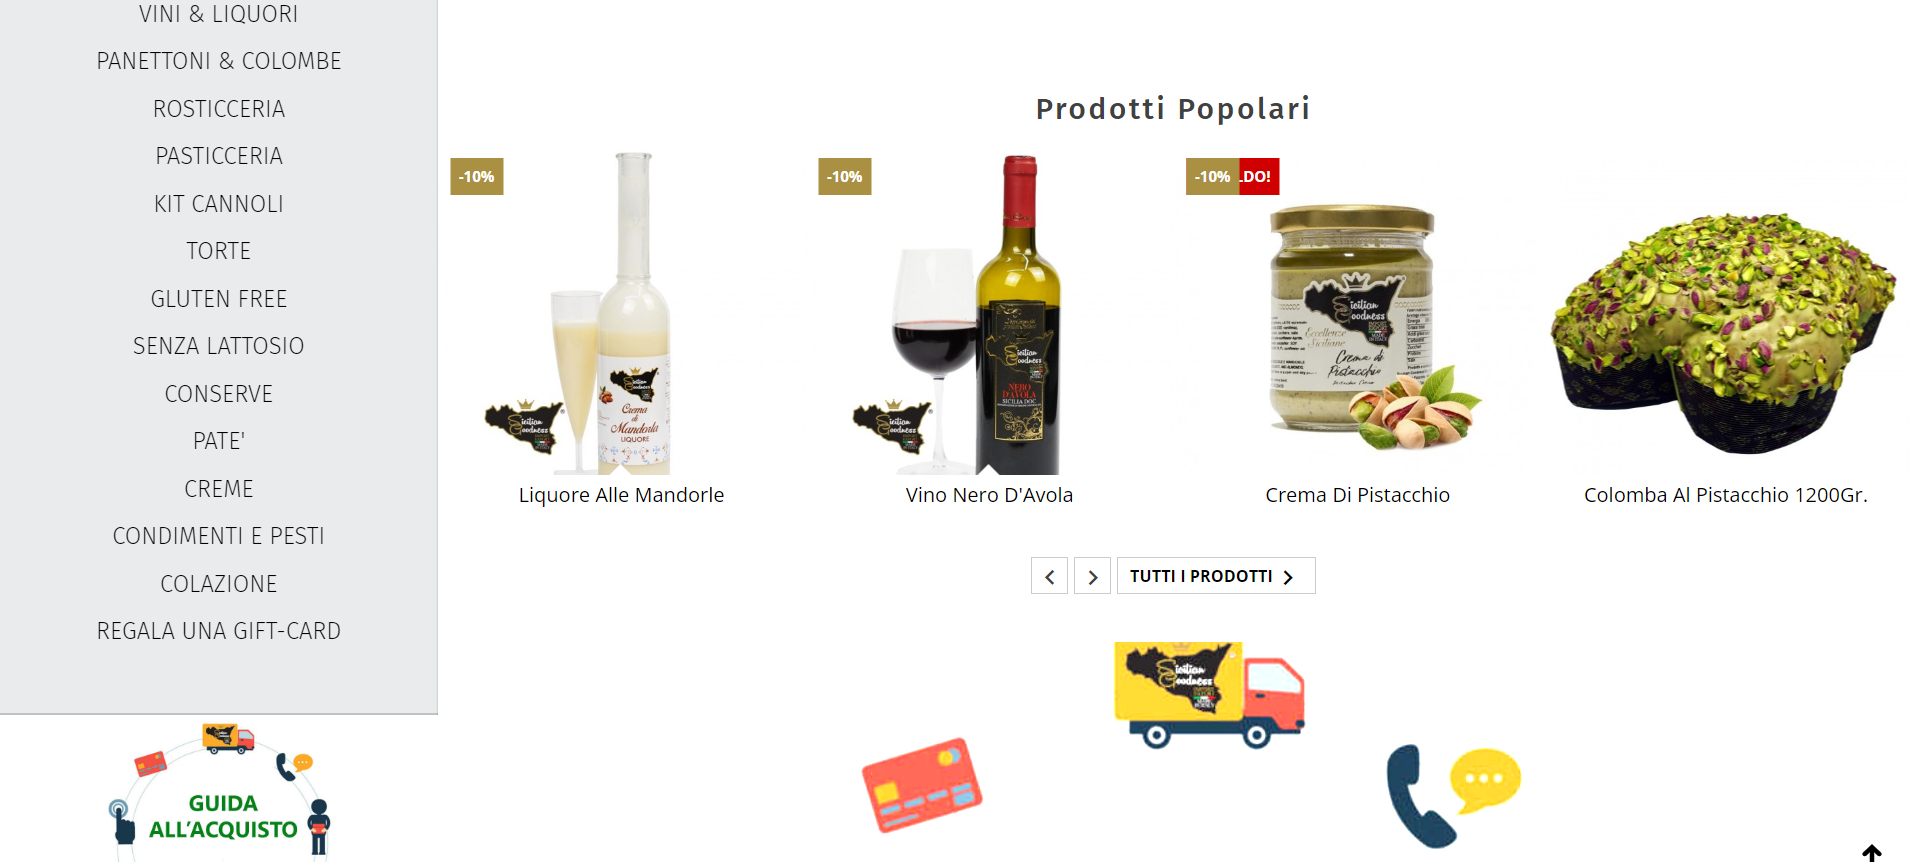
\includegraphics[width=12cm]{Img/con4.png}
	\caption{Content 4}
\end{figure}

In the fifth scroll there is an additional menu to help the user.

\begin{figure}[H]
	\centering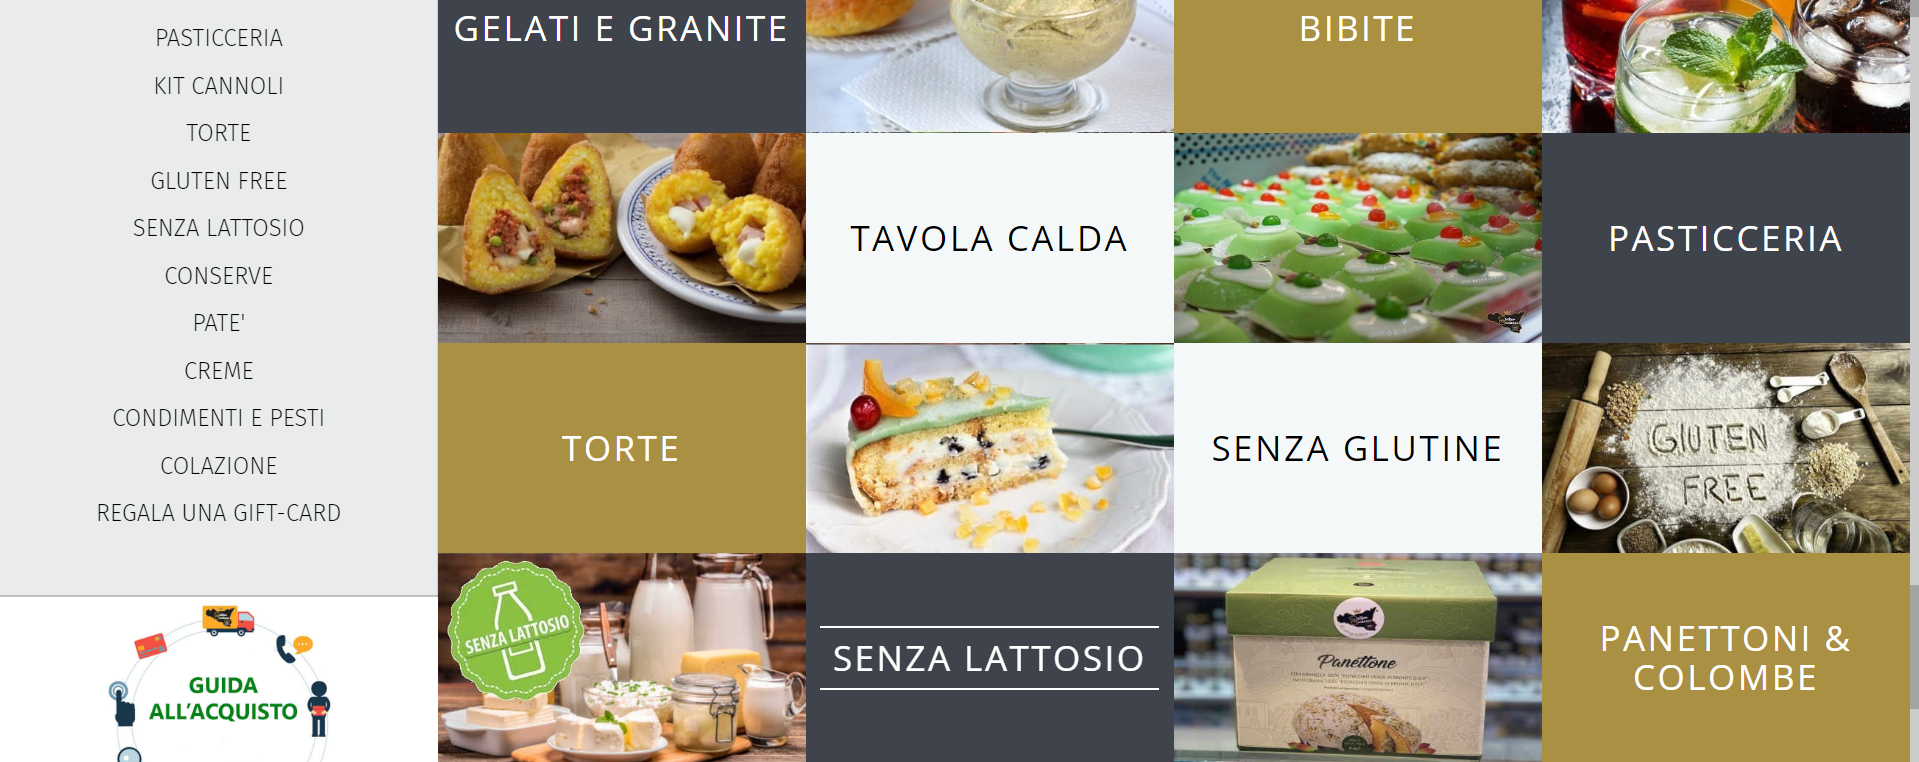
\includegraphics[width=12cm]{Img/con5.png}
	\caption{Content 5}
\end{figure}

In the last scroll we have the footer with all the information.

\begin{figure}[H]
	\centering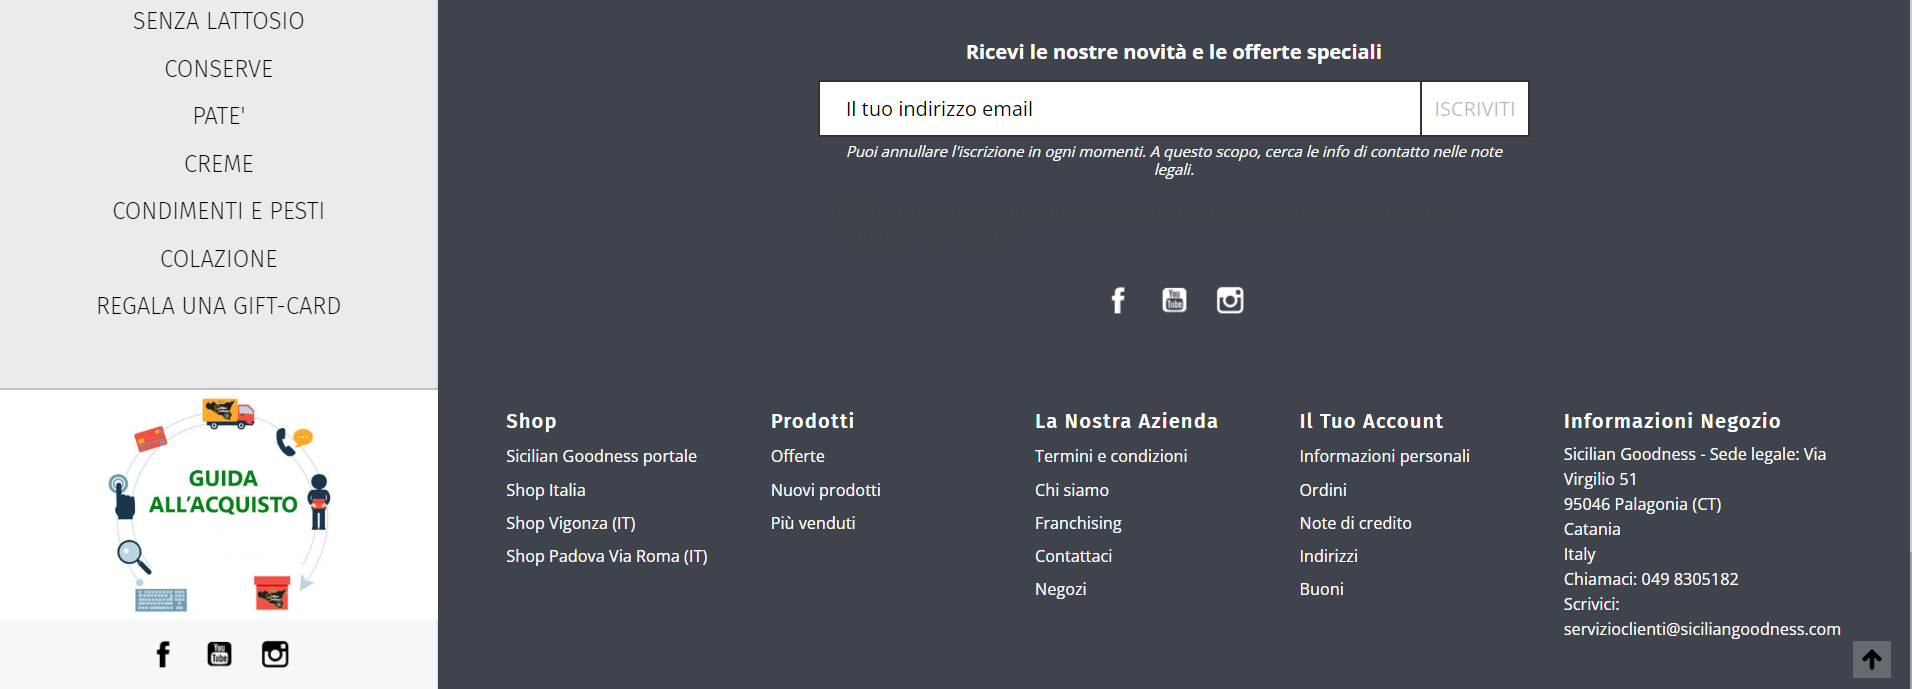
\includegraphics[width=12cm]{Img/con6.png}
	\caption{Content 6}
\end{figure}

\pagebreak

\subsection{First page} \label{sho}
In this page the logo is well situated in the top-left corner of the website.
We don't deeply analyze the Ws but we can see in the image that  mandatory axis are present(Who: in the center, Where: in the center, What: in the left column).

\begin{figure}[H]
	\centering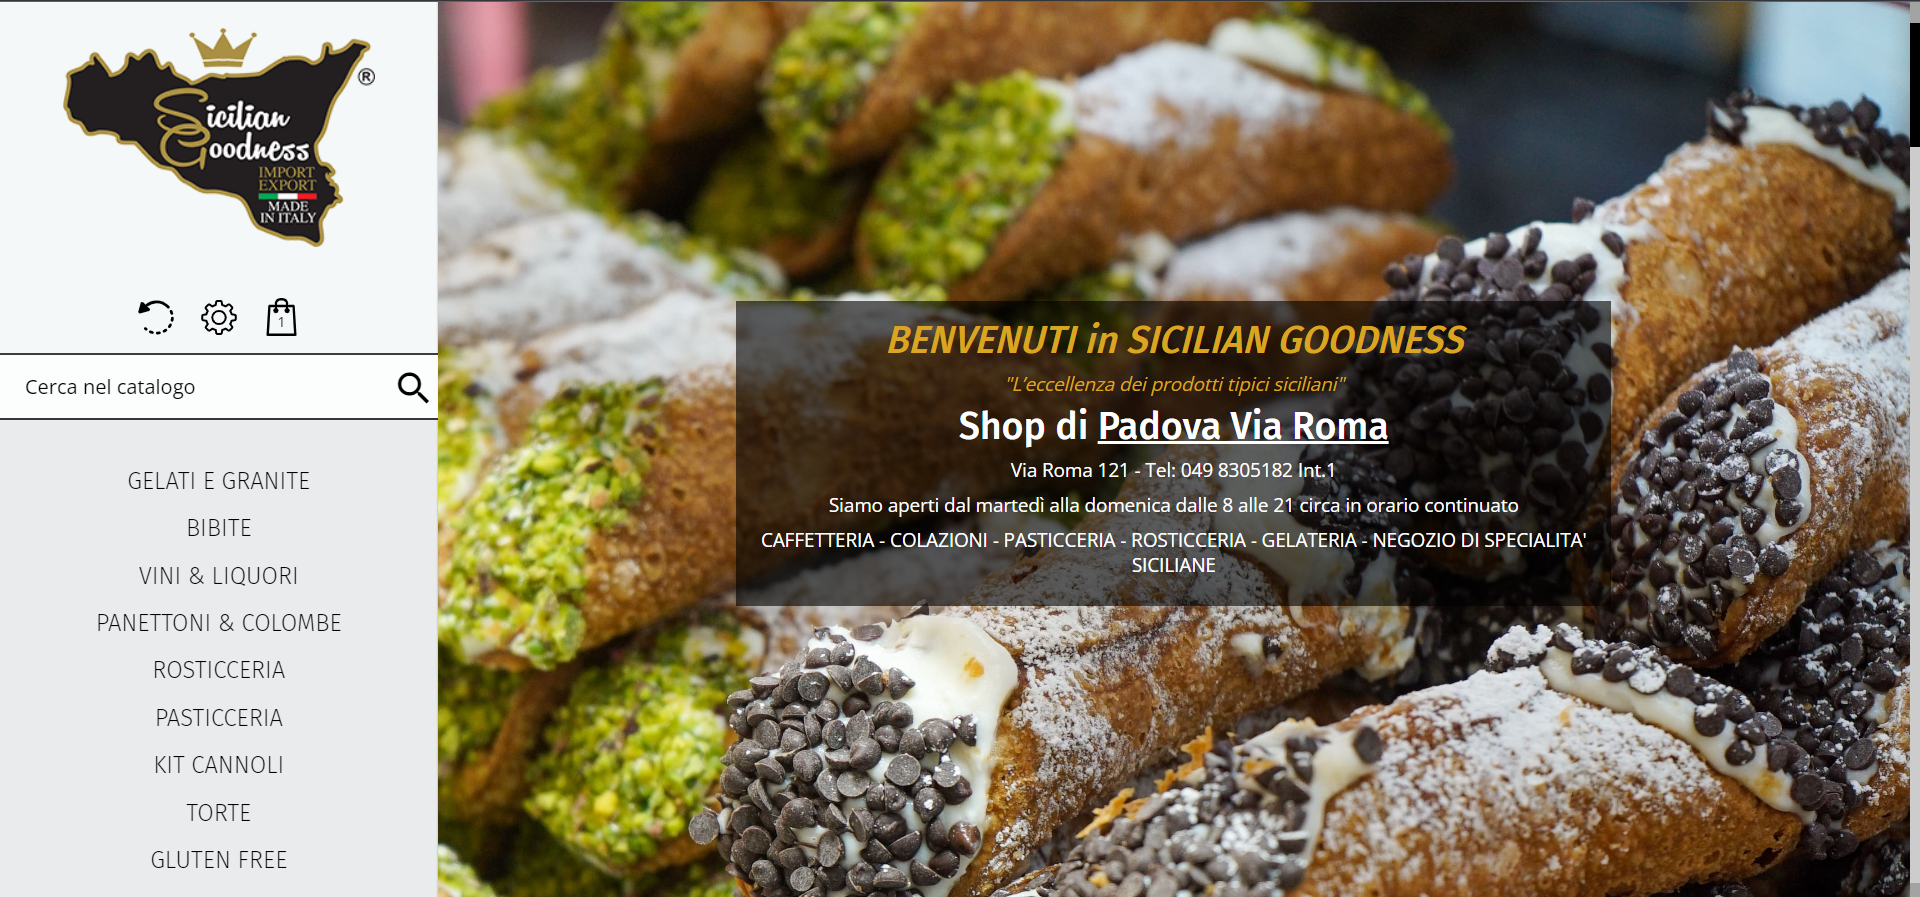
\includegraphics[width=12cm]{Img/Shop.png}
	\caption{Shop page}
\end{figure}

The menu is well structured vertically. In fact, the user can clearly search what he wants. 
Even the underlying menu is well structured. Indeed, whit its design it avoids unwanted clicks.

\begin{figure}[H]
	\centering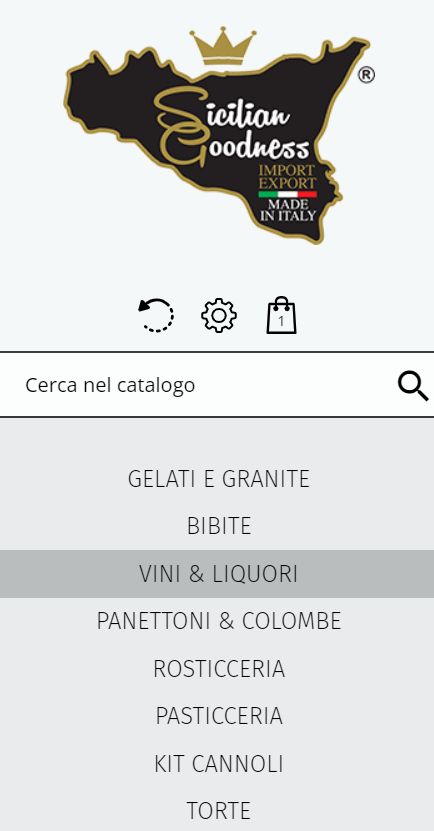
\includegraphics[height=10.5cm, width=7cm]{Img/menushop1.png}
	\caption{Menu Shop page 1}
\end{figure}

\begin{figure}[H]
	\centering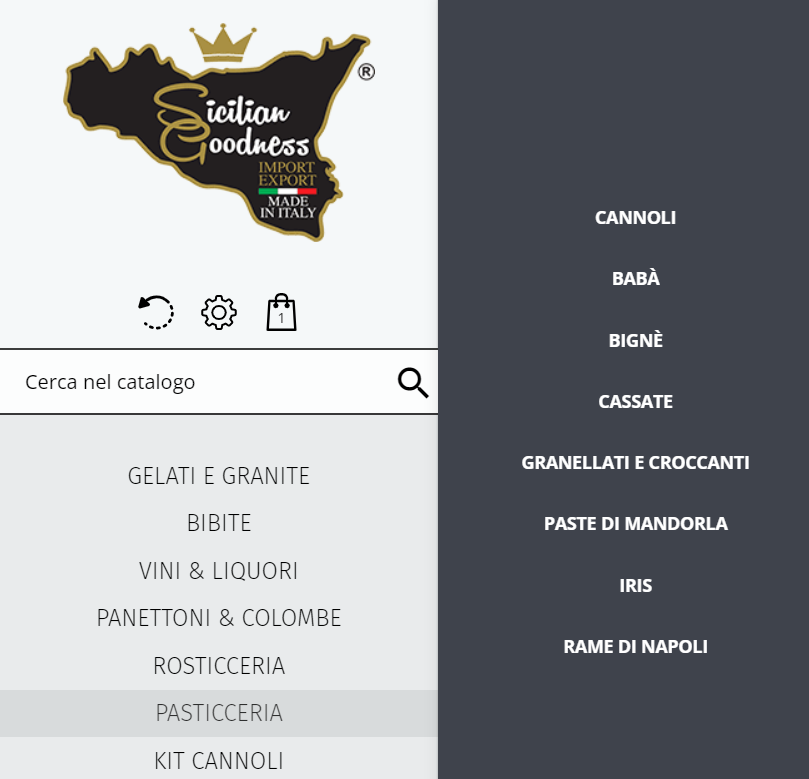
\includegraphics[height=12cm, width=12 cm]{Img/menushop2.png}
	\caption{Menu Shop page 2}
\end{figure}

To reload the page we can click on the logo or in the apposite icon under the logo.
On the right(of the previous icon) we find the registration button/icon. 
This is an other important factor because the registration is not mandatory and is not forced in any way.

\pagebreak

\subsection{Search}
Below these two icons we find the search functionality. 

\begin{figure}[H]
	\centering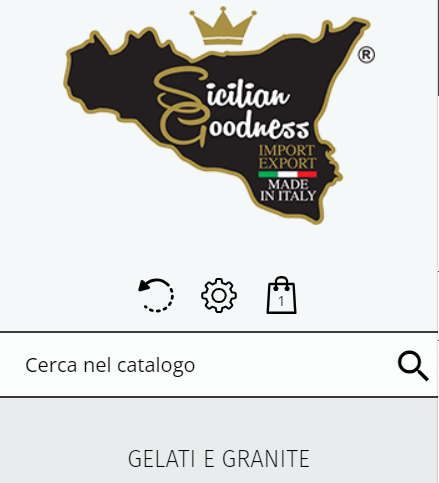
\includegraphics[height=12cm, width=10 cm]{Img/search.png}
	\caption{Search functionality}
\end{figure}

It is well structured and located in a good position.
If we use the search functionality, then we can obtain:
\begin{itemize}
	\item the results(Item);
	\item no results.
\end{itemize}

\pagebreak
  
\subsubsection{Item}
In this page we can see that the items are well locate.
Being an e-commerce, prices and products are very important.
We can observe that the website, in order to attract users, uses appropiate colors and good photos.

\begin{figure}[H]
	\centering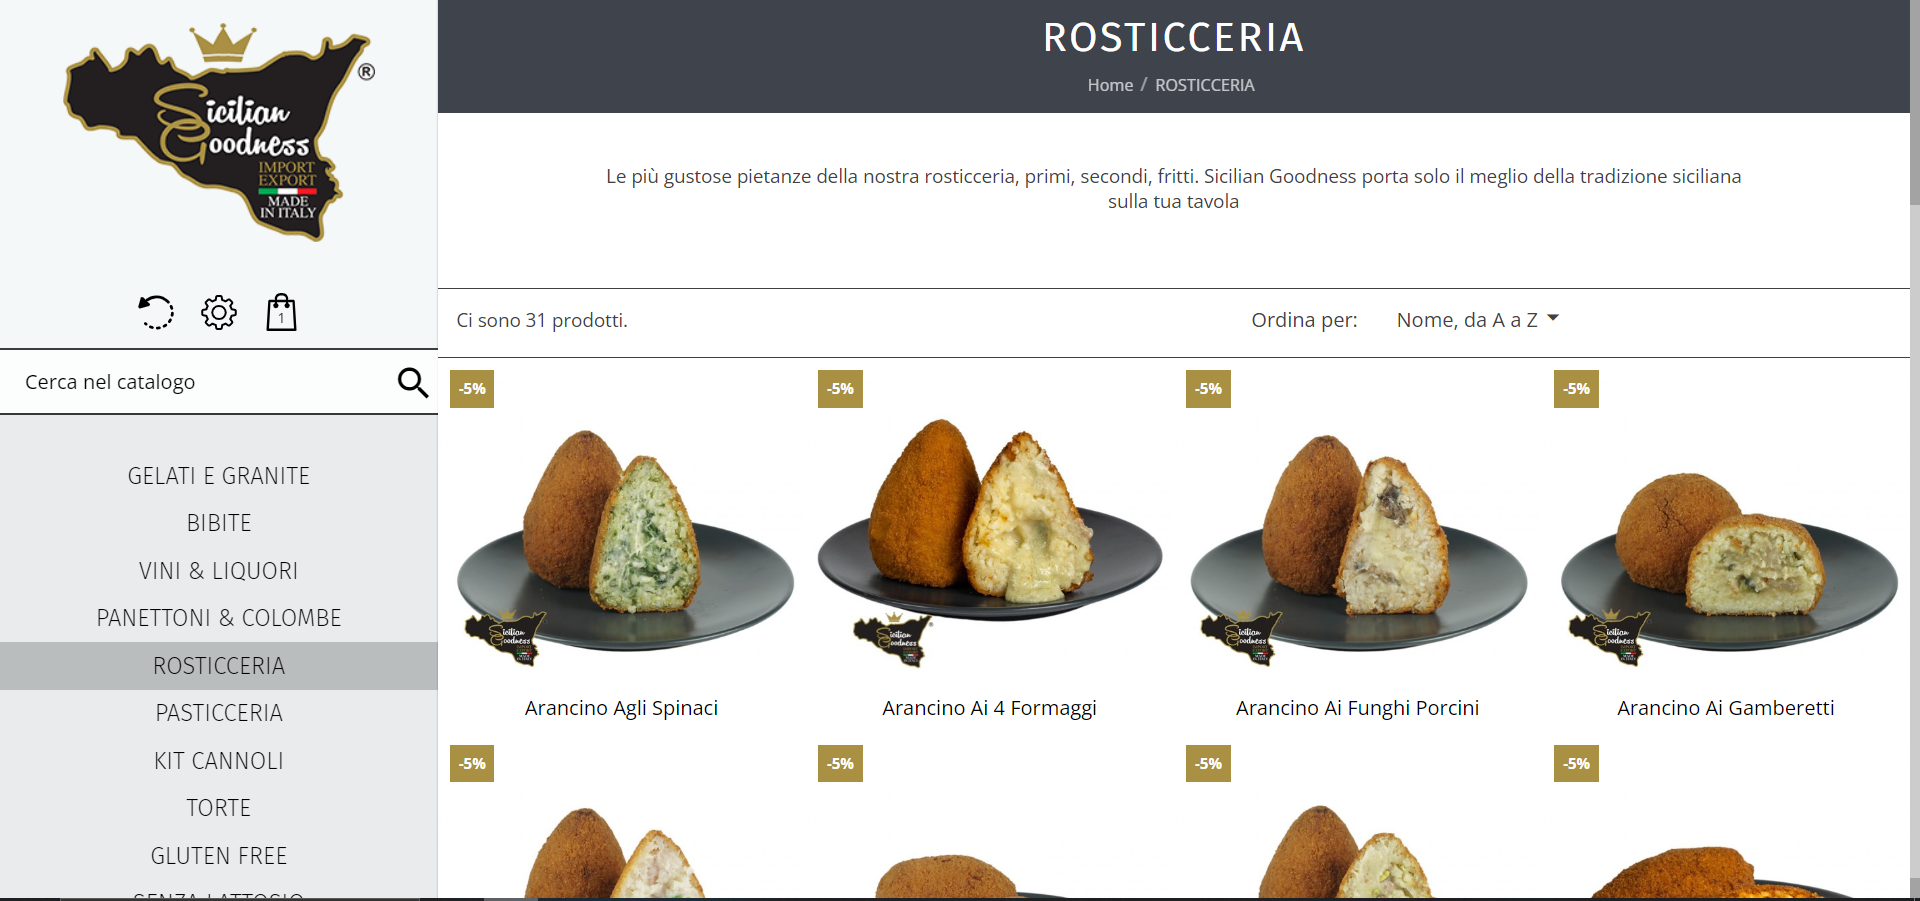
\includegraphics[width=12cm]{Img/product.png}
	\caption{Products}
\end{figure}

In this page we immediately see the percentage of discount but not the price.
The only way to see the price is the hover event and this is not too good. It is better that the price is always visible because it is one of the most important things for a user.
However, The website puts price close to the description and that is good. In addition, an other good thing is that you can see both the price and discounted price.

\begin{figure}[H]
	\centering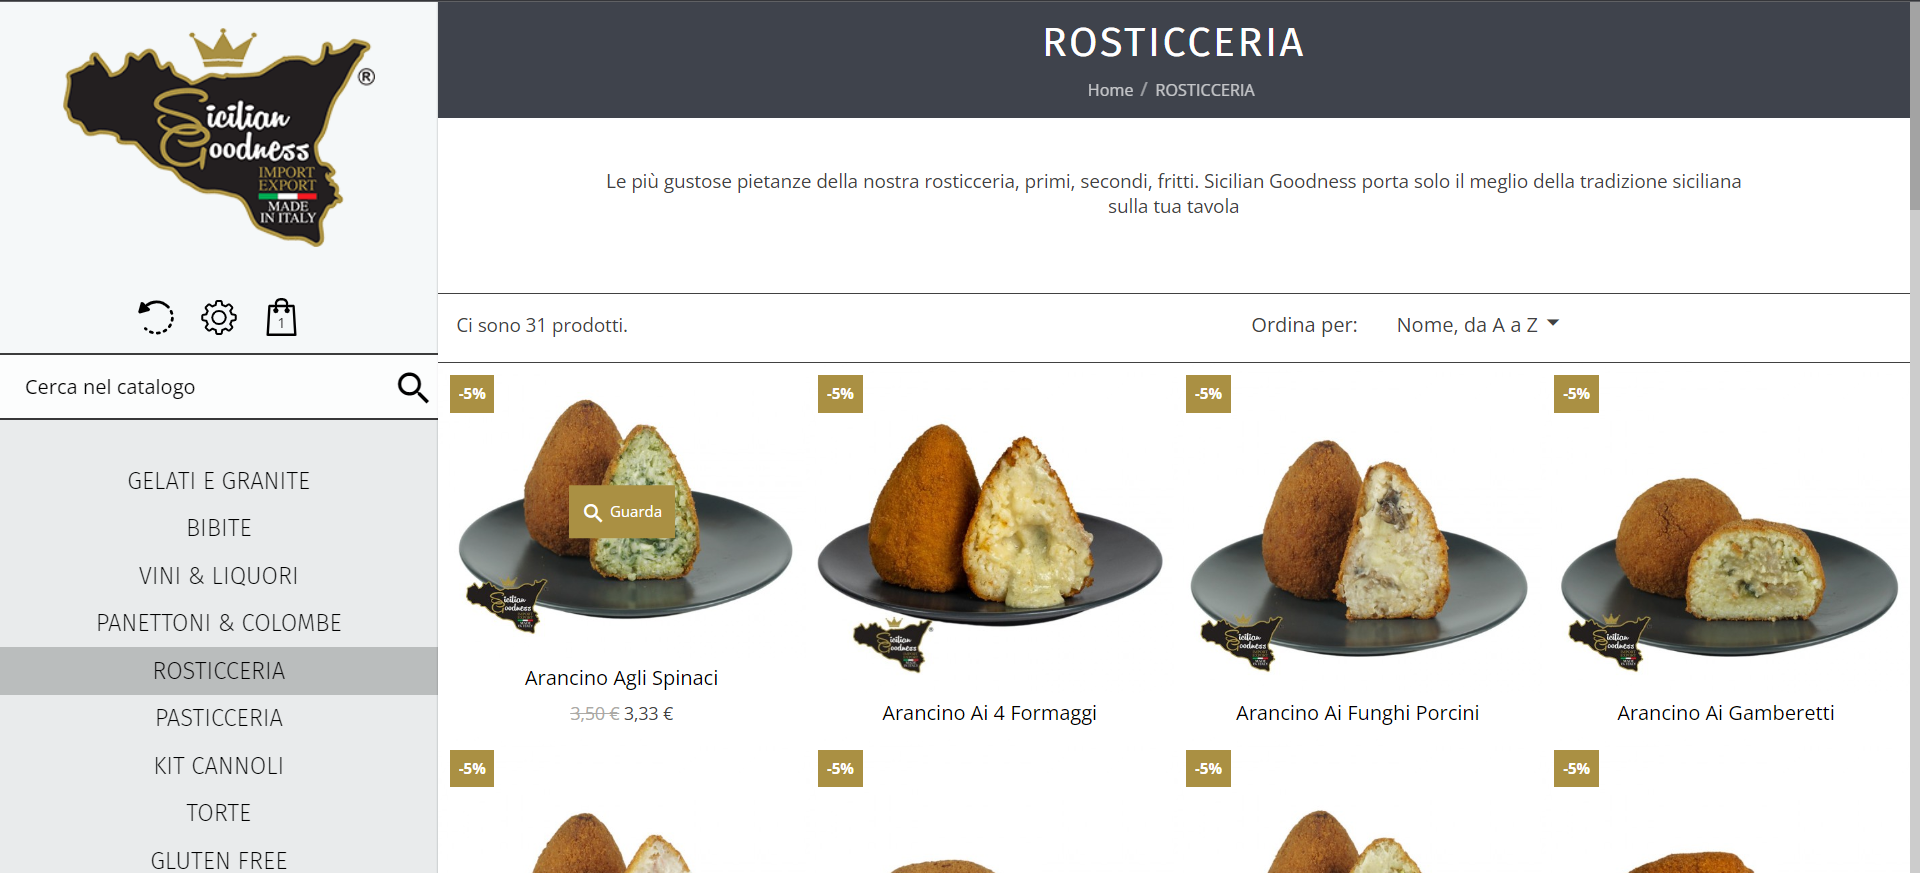
\includegraphics[width=12cm]{Img/price.png}
	\caption{Price}
\end{figure}


\subsubsection{No results}
If a product is searched through the search functionality that is not present within the site, it is displayed a clear error message.
For example we looked for 'milk' but this result doesn't exist. The website provides a good solution even if it not displays a description.

\begin{figure}[H]
	\centering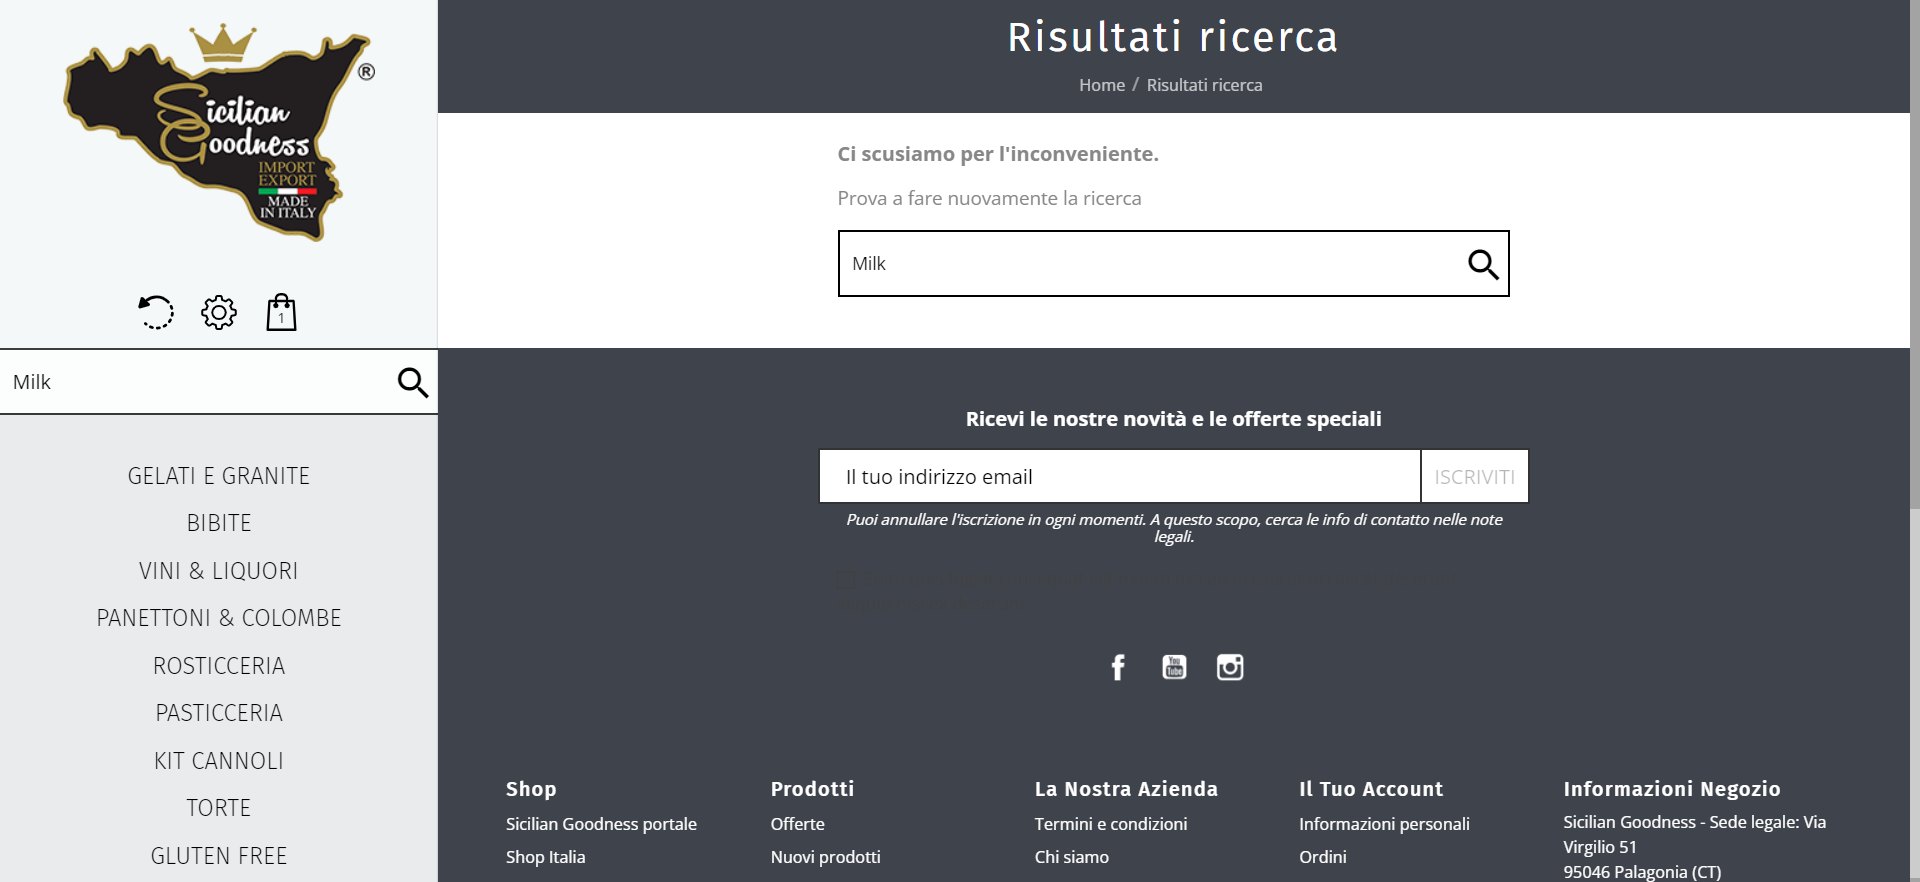
\includegraphics[width=12cm]{Img/noresult.png}
	\caption{No results page}
\end{figure}

\subsection{404}
When the average user ends up on a non-existent page, it needs simple explanations, without the use of technicalities.
If a page is searched through the URL that is not present within the site, it is displayed a clear error message.
For example we looked for \url{https://siciliangoodness.shop/padovaviaroma/vio} but this page doesn't exist. The website provides a good solution telling that the page doesn't exist.

\begin{figure}[H]
	\centering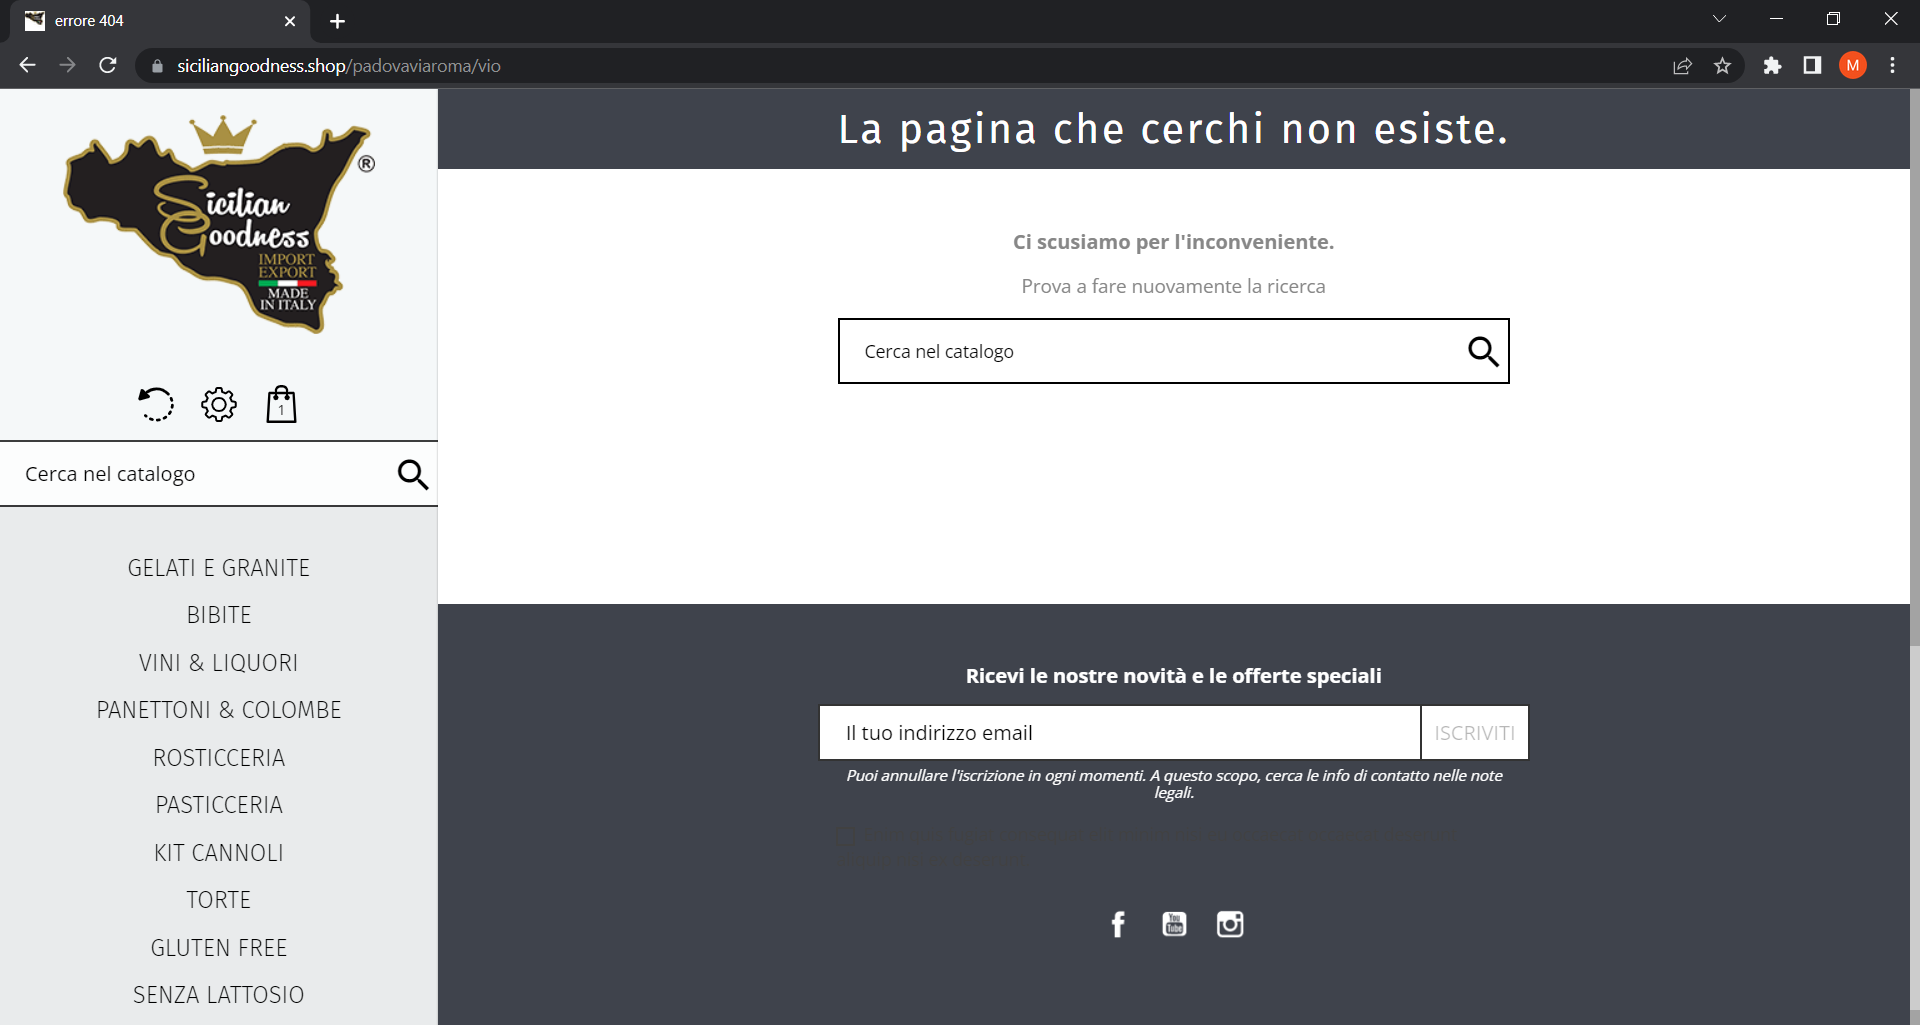
\includegraphics[width=12cm]{Img/404.png}
	\caption{404 page}
\end{figure}

\pagebreak

\subsection{Product}
The page that we analyze is \url{https://siciliangoodness.shop/padovaviaroma/rosticceria/2-arancino-al-pistacchio.html}.

\begin{figure}[H]
	\label{internalpage}
	\centering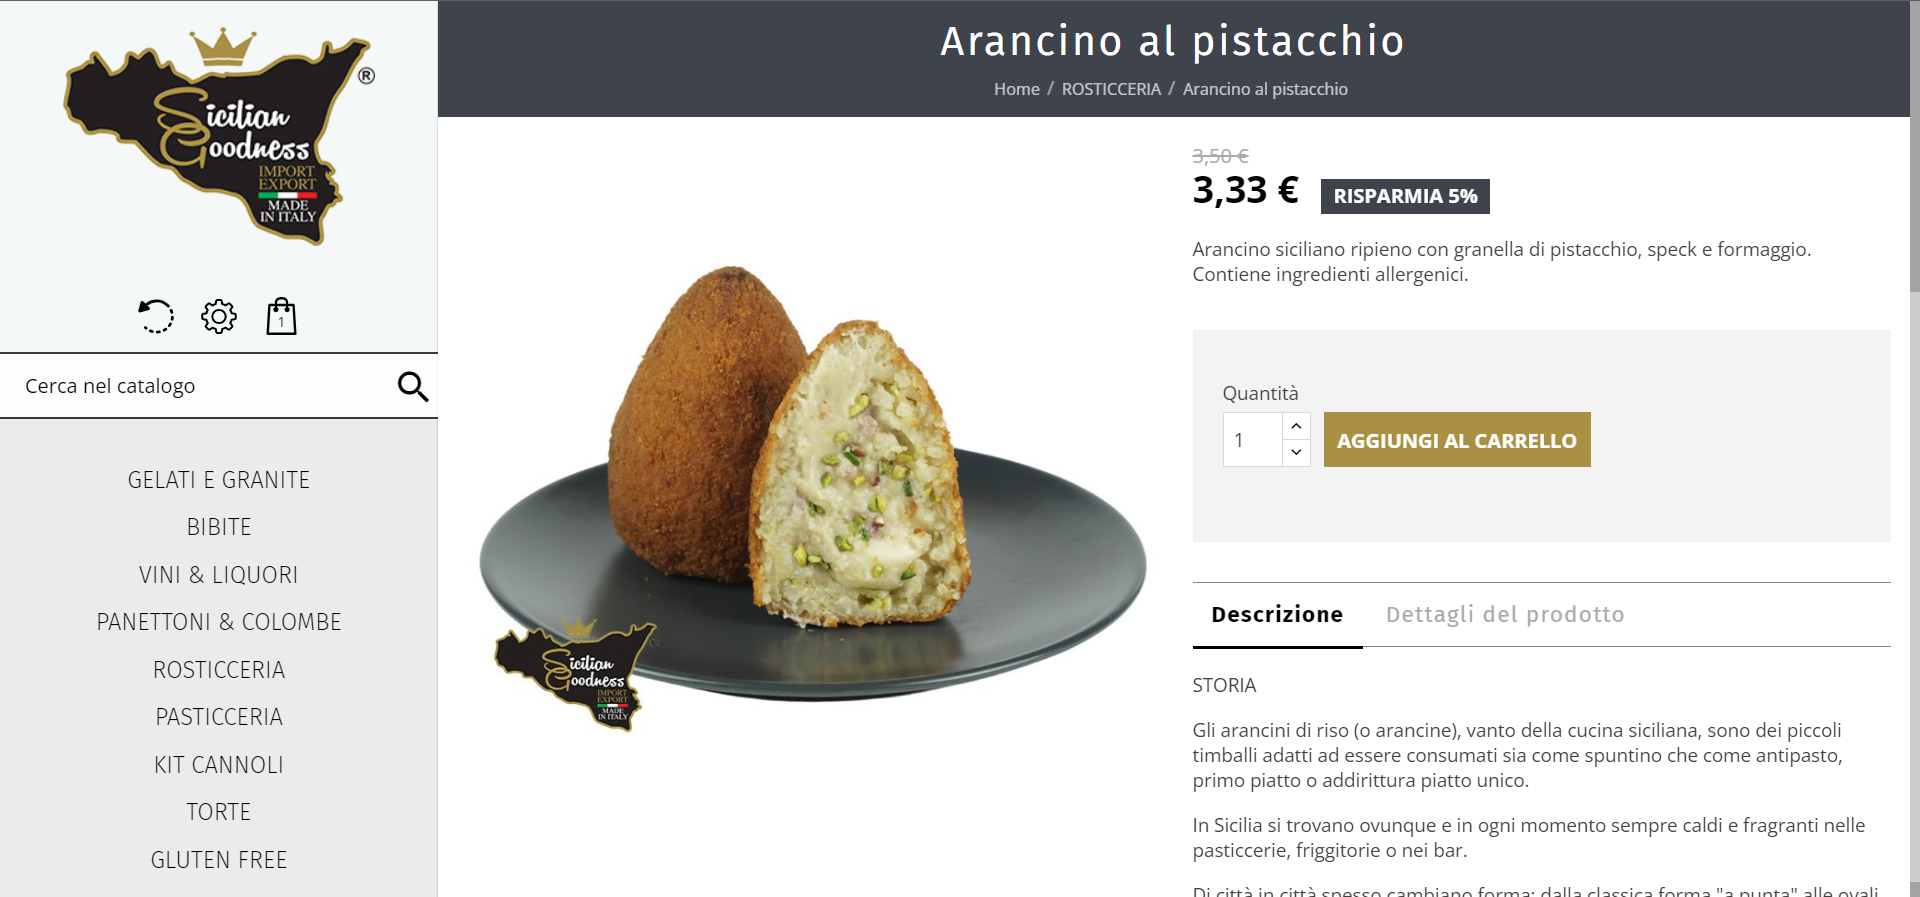
\includegraphics[width=12cm]{Img/internal.png}
	\caption{Internal page}
\end{figure}

Usually, the internal pages do not necessarily have to answer all 6 Ws:
\begin{itemize}
	\item Where: Mandatory;
	\item Who: Mandatory;
	\item What: Mandatory;
	\item When: Optional;
	\item Why: Optional;
	\item How: Optional.
\end{itemize}
As for the homepage to analyze the internal page we analyze the so-called "Six Ws".
This analysis is valid more or less for all the internal pages.

\subsubsection{The Six Ws}

\paragraph{Where}
This axis continues to have a lot of importance in the internal pages since it solves the problem of lost in navigation, allowing you to make it clear context to the user. Location breadcrumbs help to remember the path that users follow. So the Where axis is respected. 

\begin{figure}[H]
	\centering
\includegraphics[width=12cm]{Img/location.png}
	\caption{Location breadcrumb}
\end{figure}

\paragraph{Who}
Also this axis remains mandatory in internal pages, but it is sufficient to display the company logo, which Sicilian Goodness does by keeping it in the upper left corner.

\paragraph{What}
This axis remains mandatory and the presence of references to food make it clear that the theme are Sicilian procuts. The title and description help to understand the type of product.

\paragraph{When}
It is optional and this page doesn't contain any temporal reference.

\paragraph{Why}
This axis, even if it is optional, it is described very well in the section 'STORIA' as we can see in the \textbf{\hyperlink{internalpage}{Figure 35}}

\paragraph{How}
This axis is optional but it is present. In fact the search functionality is always available and we have also some tools in the footer.

\subsubsection{Cart}

The tabular display of the inserted products is very clear, where you can see the total price and the price, the discounted price with the percentage and the description of the single product. Moreover the site offers the possibility to increase the number of products or to remove items that you no longer want.

\begin{figure}[H]
	\centering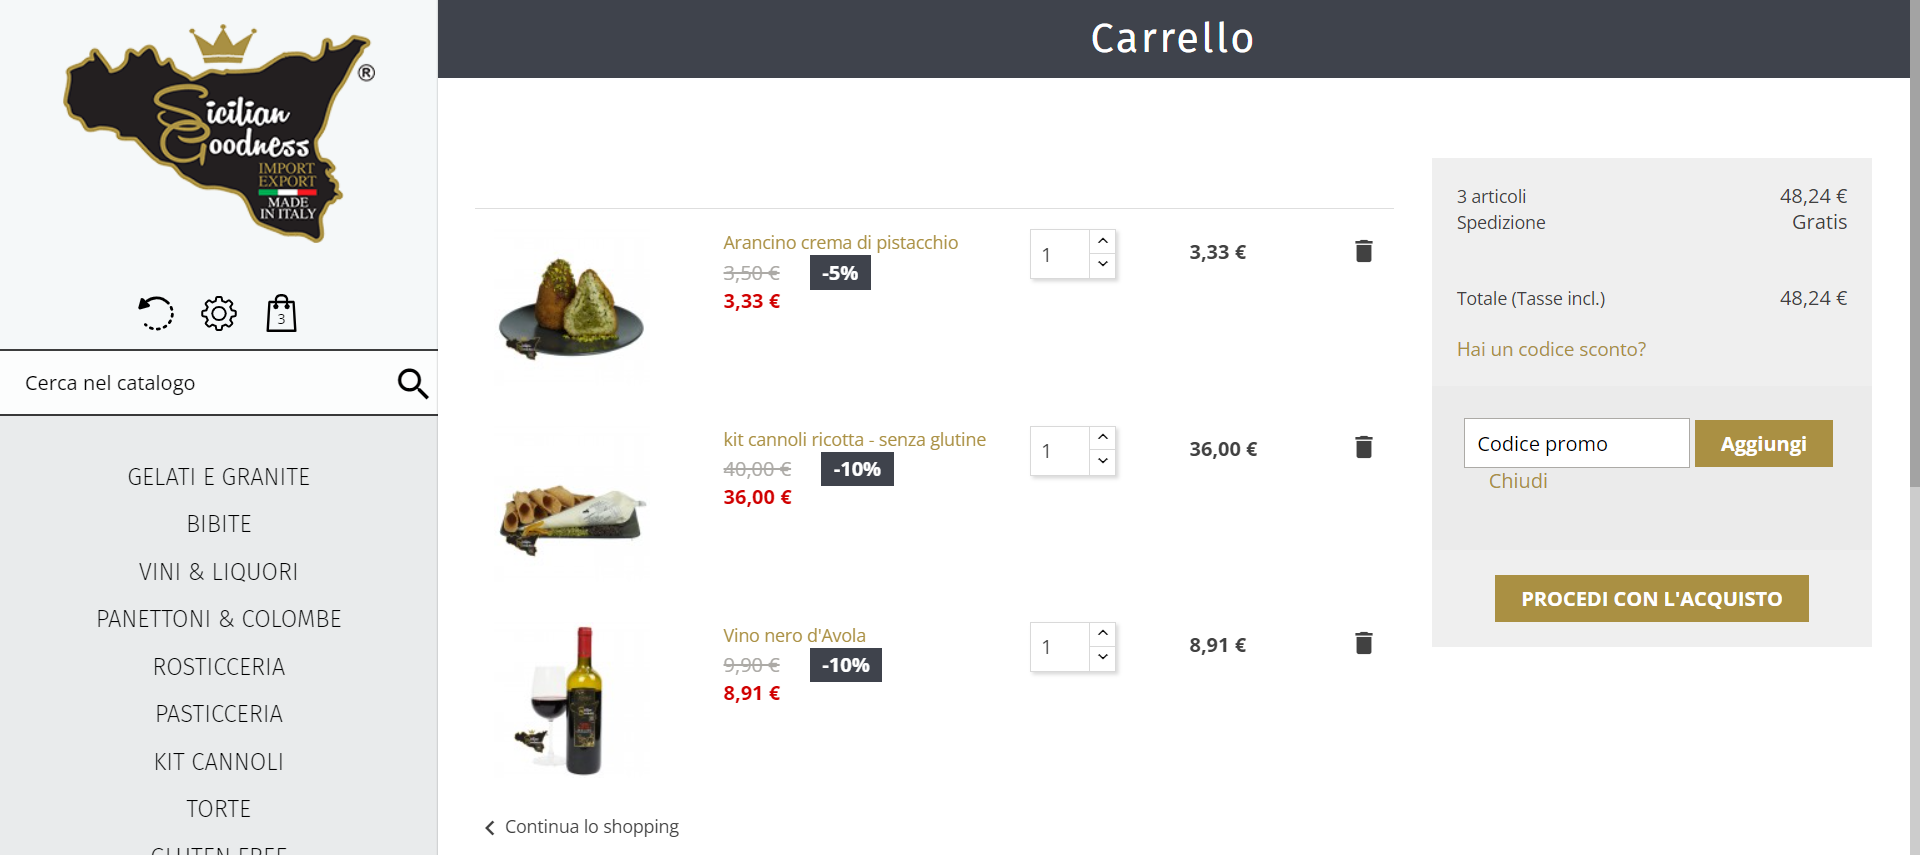
\includegraphics[width=12cm]{Img/cart.png}
	\caption{Cart}
\end{figure}

\pagebreak